\documentclass[a4paper,12pt]{scrartcl}


\usepackage[francais]{babel}
\usepackage{textcomp}
\usepackage{amsmath,amssymb}
\usepackage{lmodern}
\usepackage[a4paper]{geometry}
\usepackage{wrapfig}
\usepackage{graphicx}
\usepackage{xcolor}
\usepackage{microtype}
\usepackage{listings}
\usepackage{url}



\usepackage[utf8x]{inputenc}

\title{Vers Mercury 2.0}
\author{Quentin Cormier}



\begin{document}

\maketitle

Mercury était une fusée expérimentale développée au sein de l'association  Eureka+, et qui a volée lors du Cspace 2010.
Le but de la fusée était de mesurer le Cx de la fusée à l'aide d'un ressort sur lequel pousse le propulseur.
En fait cette expérience permet de mesurer la force de poussée du propulseur. On peut ensuite en déduire la force de résistance de l'air, puis le Cx (en connaissant la vitesse de la fusée).

Cependant le ressort à mal été dimmensionné et de nouvelles idées ont emmergés depuis le vol. Ce document montre comment choisir un ressort plus adapté, et quelles améliorations on pourrait apporter dans une seconde version de la fusée.

\section{Calcul du ressort}

\subsection{Etude théorique}
L'objectif est de déterminer quel ressort choisir, c'est à dire quelle élongation $l_0$ et quelle raideur k choisir pour pouvoir mesurer le plus précisément possible la poussée du propulseur.


En pratique $l_0$ doit être de l'ordre de 20 cm, j'essaye donc plutôt de calculer la constante k. \newpage

\begin{wrapfigure}[23]{l}{7cm}
\caption{Schéma du ressort dans le référentiel de la fusée à l'instant t}
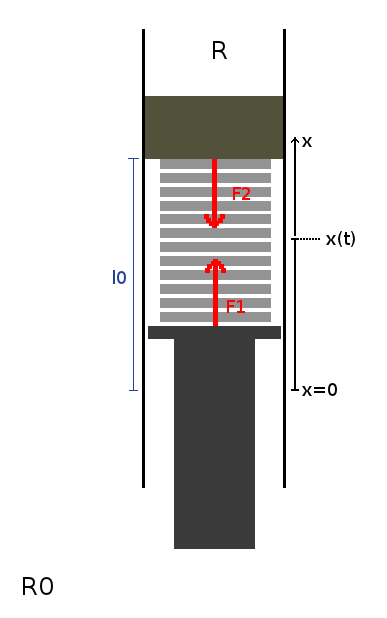
\includegraphics[width=5cm]{schema_t.png}
\end{wrapfigure}


On distingue d'abord le référentiel lié à la Terre $R_0$ Galiléen et le référentiel lié à la fusée $R$ non Galiléen.

On fait le bilan sur le ressort en appelant m sa masse, et x la position de son centre de gravité selon la longueur de la fusée, l'origine étant choisie pour correspondre au bas du ressort quand celui-ci ne subit aucune force (avant le décollage donc).

On considère ensuite que le centre de gravité du ressort est au milieu de celui-ci.
On a donc x(0) = l0 /2. 

Le ressort subit  : 
\begin{itemize}
\item $\vec{F_1}$, la force du propulseur dont le constructeur donne une courbe expérimentale en fonction du temps (c'est un PRO-54).
\item $\vec{F_2}$, la force exercée par la plaque de poussée (en verte kaki) sur le ressort
\item La force d'inertie $-m \vec{a_e}$ où $\vec{a_e}$ est l'accélération subie par la fusée en son centre de gravité dans le référentiel R0, que l'on peut donc calculer en fonction du temps avec la méthode d'Euler pour les simulations en donnant une valeur "classique" au Cx comme 0.6 (et cette accélération sera mesurée en vrai).
\item La force de Coriolis $-m\vec{\Omega} \wedge \vec{v_r}$, $\vec{\Omega}$ est la vecteur instantané de rotation donc $\vec{\Omega} = (\dot{\theta}, \dot{\varphi}, \dot{\psi})$ et $\vec{v_r}$ est la vitesse relation du ressort dans R donc $\vec{v_r} = (\dot{x}, 0, 0)$.
On a donc $\vec{\Omega} \wedge \vec{v_r} = (0, \dot{\psi} \dot{x}, \dot{\varphi} \dot{x})$.
En conclusion le produit vectoriel est nul sur l'axe des x : la force de Coriolis ne fait pas partie des forces subies par le ressort 

\item Son poids projeté sur l'axe de la fusée : $-mg*\sin{\theta}$
\end{itemize}

En écrivant le PFD sur l'axe des x, on obtient donc : $$ m\ddot{x} = F_1 - F_2 -m{a_e}_x -mg*\sin{\theta}$$ où ${a_e}_x =$ projeté de $a_e$ sur l'axe de la fusée.

En ce qui concerne F1 c'est la force du propulseur donc on peut l'estimer avec les données de poussées fournies par le constructeur du Pro-54.
En ce qui concerne F2, on déduit son expression en appliquant la troisième loi de Newton sur la plaque de poussée : $-\vec{F2}$ est la force subie par la plaque de poussée du ressort. L'allongement du ressort est $2(l0-x(t))$ donc :
$$F2 = k(l0-2x)$$


Finalement en reportant on obtient : 

$$F_{prop} + k(l0-2x) = m \ddot{x}+m{a_e}_x +mg\sin{\theta}$$ 

avec $x(0) = l0/2$.

Cette équation donne des conditions sur k.

On souhaite de plus que quand le ressort est compressé au maximum, il y ait une différence de longueur avec la longueur à vide de 7 cm : il s'agit de la différence d'élongation que l'on peut mesurer avec le potentiomètre (par exemple).

J'ai donc $2 l_0 - 2(l_0-max(x)) = 7cm$ ie : $$max(x) = 3.5 cm$$


Ceci est donc une contrainte supplémentaire sur k.

\subsection{Simulation numérique}

Pour trouver la valeur de k et calculer la position théorique du ressort à tout instant, on réalise une simulation numérique en Ocaml\footnote{Très bon langage de programmation enseigné en prépa}.

On calcule les différentes valeurs en donnant une valeur classique au $C_x$ de 0.6.
On calcule d'abord la position et l'accélération de la fusée sur sa longeur, ce qui correspont à ${a_e}$ puis la position du ressort à tout instant.

Le code complet du programme peut être visionné ici : \url{https://github.com/robocop/Mercury}

\subsection{Résultats}

Pour la fusée qui a volé, on trouve k = 11880 N soit 5 fois plus que le ressort que nous avions choisit : 
\begin{lstlisting}
$ ./calculs.native 
k = 11882.324219 N.m^-1
t : 0.315000 	 h = 3.941081 	 v = 27.242454 	 theta = 79 	 a = 91.197535 
t : 15.730000 	 h = 1328.005704 	 v = 24.011964 	 theta = 0	 a = -0.343766 
\end{lstlisting}

A la place du ressort, on pourrait utiliser un capteur de distance infrarouge comme les Sharp gp2d120 pouvant mesurer une distance de 
4 à 30 cm.

On peut alors choisir un ressort de 30 cm et une différence d'élongation de 15 cm : 
\begin{lstlisting}
$ ./calculs.native -l0 0.3 -l_potar 0.15
k = 6046.295166 N/m
t : 0.315000 	 h = 3.941081 	 v = 27.242454 	 theta = 79 	 a = 91.197535 
t : 15.730000 	 h = 1328.005704 	 v = 24.011964 	 theta = 0 	 a = -0.343766 
\end{lstlisting}

\end{document}